\documentclass[springer.tex]{subfiles}
\graphicspath{ {./figures/} }

\begin{document}
\chapter{Mutable values}
\section{Variables}
\label{sec:mutableValues}
Identifiers may be mutable, which means that the it may be rebound to a new value. Mutable identifiers are specified using the \idx[mutable@\lstinline{mutable}]{\keyword{mutable}} keyword with the following syntax:
%
\begin{verbatimwrite}{\ebnf/variables.ebnf}
let mutable <*ident*> = <*expr*> [*in <*expr*>*]
\end{verbatimwrite}
\syntax{\ebnf/variables.ebnf}{Syntax for defining mutable values with an initial value.}
%
Changing the value of an identifier is called \idx{assignment} and is done using the \idx[{<-}@\lstinline{<-}]{\lexeme{<-}} lexeme. Assignments have the following syntax:\jon{Discussion on heap and stack should be added here.}
%
\begin{verbatimwrite}{\ebnf/assignment.ebnf}
<*ident*> <- <*ident*>
\end{verbatimwrite}
\syntax{\ebnf/assignment.ebnf}{Value reassignment for mutable variables.}
%
\idx[mutable value]{Mutable values} is synonymous with the term \idx{variable}. A variable is an area in the computer's working memory associated with an identifier and a type, and this area may be read from and written to during program execution, see \Cref{mutableAssignReassingShort} for an example.
%
\fs{mutableAssignReassingShort}{A variable is defined and later reassigned a new value.}
%\fs{mutableAssignReassing}{}
%
Here, an area in memory was denoted \lstinline{x}, initially assigned the integer value 5, hence the type was inferred to be \lstinline|int|.  Later, this value of \lstinline{x} was replaced with another integer using the \lexeme{<-} lexeme. The \lexeme{<-} lexeme is used to distinguish the assignment from the comparison operator. For example, the statement \lstinline{a = 3} in \Cref{mutableEqual} is not an assignment but a comparison which is evaluated to be false. 
%
\fsOutput{mutableEqual}{It is a common error to mistake \lexeme{=} and \lexeme{<-} lexemes for mutable variables.}
% \begin{lstlisting}[language=fsharp,caption={fsharpi, example of changing the content of a variable.}]
% > let mutable a = 0
% - a = 3;;
%
% val mutable a : int = 0
% val it : bool = false
% \end{lstlisting}
%
However, it is important to note that when the variable is initially defined, then the '\lexeme{=}' operator must be used, while later reassignments must use the \lexeme{<-} expression.

Assignment type mismatches will result in an error, as demonstrated in \Cref{mutableAssignReassingTypeError}. 
%
\fs{mutableAssignReassingTypeError}{Assignment type mismatching causes a compile-time error.}
%
I.e., once the type of an identifier has been declared or inferred, it cannot be changed.

A typical variable is a counter of type integer, and a typical use of counters is to increment them, see \Cref{mutableAssignIncrement} for an example.
%
\fs{mutableAssignIncrement}{Variable increment is a common use of variables.}
%
Using variables in expressions, as opposed to the left-hand-side of an assignment operation, reads the value of the variable. Thus, when using a variable as the return value of a function, then the value is copied from the local scope of the function to the scope from which it is called. This is demonstrated in \Cref{mutableAssignReturnVariable}.
%
\fsOutput{mutableAssignReturnVariable}{Returning a mutable variable returns its value.}
%
In the example we see that the type is a value, and not mutable. 

Variables implement dynamic scope, that is, the value of an identifier depends on \emph{when} it is used. This is in contrast to lexical scope, where the value of an identifier depends on \emph{where} it is defined. As an example, consider the script in \Cref{lexicalScopeNFunction} which defines a function using lexical scope and returns the number \lstinline!6.0!, however, if \lstinline!a! is made \lstinline!mutable!, then the behavior is different, as shown in \Cref{dynamicScopeNFunction}.
%
\fs{dynamicScopeNFunction}{Mutual variables implement dynamic scope rules. Compare with \Cref{lexicalScopeNFunction}.}
%
Here, the response is \lstinline!8.0!, since the value of \lstinline!a! changed before the function \lstinline!f! was called.

\section{Reference Cells}
\label{sec:referenceCells}
%F\# has a variation of mutable variables called \idx{reference cells}. Reference cells have built-in function \idx[ref@\lstinline{ref}]{\lstinline{ref}} and operators \idx[{!}@\lstinline{!}]{\lexeme{!}} and \idx[{:=}@\lstinline{:=}]{\lexeme{:=}}, where \lstinline{ref} creates a reference variable, and the '\lexeme{!}' and the '\lexeme{:=}' operators reads and writes its value. An example of using reference cells is given in \Cref{refCell}.
F\# has a variation of mutable variables called \idx{reference cells}. Reference cells have the built-in function \idx[ref@\lstinline{ref}]{\lstinline{ref}} and the operators \lexeme{!} and \idx[{:=}@\lstinline{:=}]{\lexeme{:=}}, where \lstinline{ref} creates a reference variable, and the '\lexeme{!}' and the '\lexeme{:=}' operators respectively reads and writes its value. An example of using reference cells is given in \Cref{refCell}.
%
\fs{refCell}{Reference cells are variants of mutable variables.}
%
Reference cells are different from mutable variables, since their content is allocated on \idx{The Heap}. The Heap is a global data storage that is not destroyed when a function returns, which is in contrast to the \idx{call stack}, also known as \idx{The Stack}. The Stack maintains all the local data for a specific instance of a function call, see \Cref{sec:callStack} for more details. As a consequence, when a reference cell is returned from a function, then it is the reference to the location on The Heap, which is returned as a value. Since this points outside the local data area of the function, this location is still valid after the function returns, and the variable stored there is accessible to the caller. This is illustrated in \Cref{fig:returningRefCells}
%
\begin{figure}
  \centering
  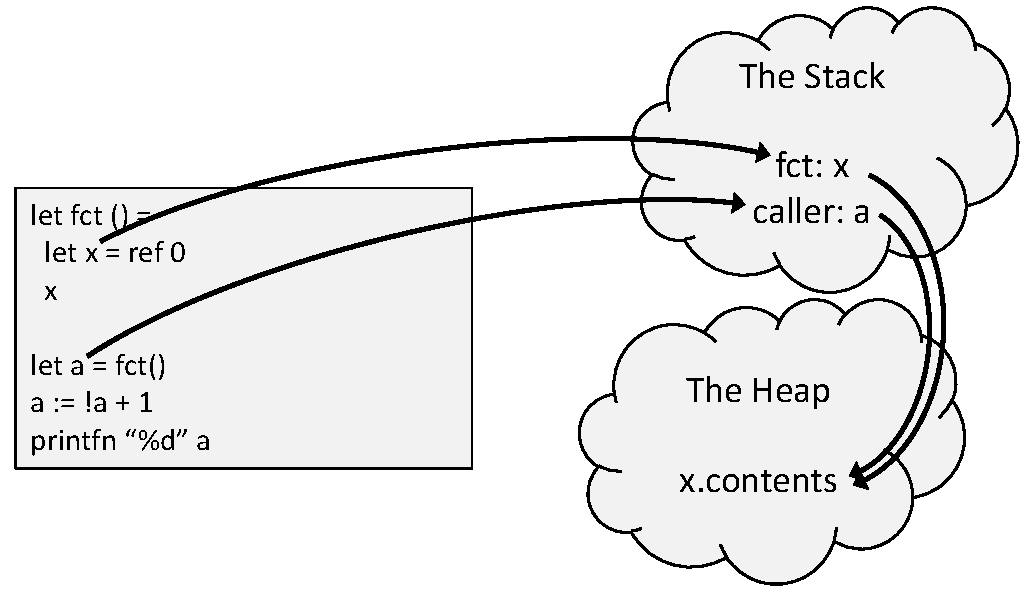
\includegraphics[width=0.6\textwidth]{ReferenceCells}
  \caption{A reference cell is a pointer to The Heap, and the content is not destroyed when its reference falls out of scope.}
  \label{fig:returningRefCells}
\end{figure}
%

Reference cells may cause \idx[side-effect]{side-effects}, where variable changes are performed across independent scopes. Some side-effects are useful, e.g., the \lstinline{printf} family changes the content of the screen, and the screen is outside the scope of the caller.  Another example of a useful side-effect is a counter shown in \Cref{refEncapsulation}.
%
\fs{refEncapsulation}{An increment function with a local state using a reference cell.}
%
Here \lstinline{incr} is an anonymous function with an internal state \lstinline{counter}. At first glance, it may be surprising that \lstinline{incr ()} does not return the value \lstinline{1} at every call. The reason is that the value of the \lstinline{incr} is the closure of the anonymous function \lstinline{fun () -> counter := ...}, which is 
\begin{equation}
  \text{\lstinline{incr}}: \left(\text{args}, \text{exp}, \text{env}\right)  = \big((), \left(\begin{subarray}{l}\displaystyle\text{\lstinline{counter := !counter + 1}}\\\displaystyle\text{\lstinline{!counter}}\end{subarray}\right), (\text{\lstinline{counter}}\rightarrow\text{\lstinline{ref 0}})\big).
\end{equation}
Thus, \lstinline{counter} is only initiated once at the initial binding, while every call of \lstinline{incr ()} updates its value on The Heap. Such a programming structure is called \idx{encapsulation}, since the \lstinline{counter} state has been encapsulated in the anonymous function, and the only way to access it is by calling the same anonymous function. In general, it is advisable to \advice{use encapsulation to hide implementation details irrelevant to the user of the code.}

The \lstinline{incr} example in \Cref{refEncapsulation} is an example of a useful side-effect. An example to be avoided is shown in \Cref{refSideEffect}.
%
\fs{refSideEffect}{Intertwining independent scopes is typically a bad idea.}
%
In the example, the function \lstinline{updateFactor} changes a variable in the scope of the function \lstinline{multiplyWithFactor}. The code style is prone to errors, since the computations are not local at the place of writing, i.e., in \lstinline{multiplyWithFactor}, and if \lstinline{updateFactor} were defined in a library, then the source code may not be available. Better style of programming is shown in \Cref{refWithoutSideEffect}.
%
\fs{refWithoutSideEffect}{A solution similar to \Cref{refSideEffect} without side-effects.}
%
Here, there can be no doubt in \lstinline{multiplyWithFactor} that the value of \lstinline{a} is changing. Side-effects do have their use, but should, in general, be avoided at almost all costs, and it is advised to \advice{minimize the use of side effects}.

Reference cells give rise to an effect called \idx{aliasing}, where two or more identifiers refer to the same data, as illustrated in \Cref{refCellAliasing}.
%
\fs{refCellAliasing}{Aliasing can cause surprising results and should be avoided.}
%
Here, \lstinline!a! is defined as a reference cell, and by defining \lstinline!b! to be equal to \lstinline!a!, we have created an alias. This can be very confusing since as the example shows, changing the value of \lstinline!b! causes \lstinline!a! to change as well. Aliasing is a variant of side-effects, and \advice{aliasing should be avoided at all costs}.

Since F\# version 4.0, the compiler has automatically converted mutable variables to reference cells, where needed.  E.g., \Cref{refEncapsulation} can be rewritten using a mutable variable, as shown in \Cref{mutableEncapsulation}.
% 
\fs{mutableEncapsulation}{Local mutable content can be indirectly accessed outside its scope.}
% 
Reference cells are preferred over mutable variables for encapsulation, in order to avoid confusion.

\section{Arrays}
\label{sec:arrays}
One dimensional \idx{arrays}, or just arrays for short, are mutable lists of the same type and follow a similar syntax as lists. Arrays can be stated as a \idx{sequence expression},
%
\begin{verbatimwrite}{\ebnf/arrays.ebnf}
[|[*<*expr*>{*; <*expr*>*}*]|]
\end{verbatimwrite}
\syntax{\ebnf/arrays.ebnf}{The syntax for an array using the sequence expression.}
%
E.g., \mbox{\lstinline![|1; 2; 3|]!} is an array of integers, \mbox{\lstinline![|"This"; "is"; "an"; "array"|]!} is an array of strings, \mbox{\lstinline![|(fun x -> x); (fun x -> x*x)|]!} is an array of functions, \lstinline![||]! is the empty array.  Arrays may also be given as ranges,
%
\begin{verbatimwrite}{\ebnf/arrayRange.ebnf}
[|<*expr*> .. <*expr*> [*.. <*expr*>*]|]
\end{verbatimwrite}
\syntax{\ebnf/arrayRange.ebnf}{The syntax for an array using the range expression.}
%
but arrays of \idx{range expressions} must be of \lstinline[language=syntax]{<*expr*>} integers, floats, or characters. Examples are \mbox{\lstinline![|1 .. 5|]!}, \mbox{\lstinline![|-3.0 .. 2.0|]!}, and \mbox{\lstinline![|'a' .. 'z'|]!}. Range expressions may include a step size, thus, \mbox{\lstinline![|1 .. 2 .. 10|]!} evaluates to \mbox{\lstinline![|1; 3; 5; 7; 9|]!}.

The array type is defined using the \keyword{array} keyword or alternatively the \lexeme{[]} lexeme.  Like strings and lists, arrays may be indexed using the \idx[{.[]}@\lstinline{.[]}]{\lexeme{.[]}} notation. Arrays cannot be resized, but are mutable, as shown in \Cref{arrayReassign}.
%
\fs{arrayReassign}{Arrays are mutable in spite of the missing \keyword{mutable} keyword.}
%
Notice that in spite of the missing \keyword{mutable} keyword, the function \lstinline{square} still has the \idx{side-effect} of squaring all entries in \lstinline{A}.  F\# implements arrays as chunks of memory and indexes arrays via address arithmetic. I.e., element $i$ in an array, whose first element is in memory address $\alpha$ and whose elements fill $\beta$ addresses each, is found at address $\alpha+i\beta$.\jon{Add a figure illustrating address indexing.} Hence, indexing has computational complexity of $\mathcal{O}(1)$, but appending and prepending values to arrays and array concatenation requires copying the new and existing values to a fresh area in memory and thus has computational complexity $\mathcal{O}(n)$, where $n$ is the total number of elements. Thus, \advice{indexing arrays is fast, but cons and concatenation is slow and should be avoided.}

Arrays support \idx{slicing}, that is, indexing an array with a range result in a copy of the array with values corresponding to the range. This is demonstrated in \Cref{arraySlicing}.
%
\fsOutput{arraySlicing}{Examples of array slicing. Compare with \Cref{listSlicing} and \Cref{stringIndexing}.}
%
As illustrated, the missing start or end index imply from the first or to the last element, respectively.

Arrays do not have explicit operator support for appending and concatenation, instead the \lstinline{Array} namespace includes an \lstinline{Array.append} function, as shown in \Cref{arrayAppend}.
%
\fs{arrayAppend}{Two arrays are appended with \lstinline{Array.append}.}
%

Arrays are \idx{reference types}, meaning that identifiers are references and thus suffer from aliasing, as illustrated in \Cref{arrayAliasing}.
%
\fs{arrayAliasing}{Arrays are reference types and suffer from aliasing.}
%
\clearpage

\subsection{Array Properties and Methods}
\label{sec:arrayMethods}
Some important properties and methods for arrays are:
\begin{description}
\item[\texttt{Clone()}:] \lstinline{'T []}.~\\
  Returns a copy of the array.
  \fsOutputNF{arrayCloneProp}{\lstinline{Clone}}\idxss{Clone@\lstinline{Clone}}
\item[\texttt{Length}:] \lstinline{int}.~\\
  Returns the number of elements in the array.
  \fsOutputNF{arrayLengthProp}{\lstinline{Length}}\idxss{Length@\lstinline{Length}}
\end{description}

\subsection{The Array Module}
There are quite a number of built-in procedures for arrays in the \lstinline{Array} module, some of which are summarized below.
\begin{description}
\item[\texttt{Array.append}:] \lstinline{arr1:'T [] -> arr2:'T [] -> 'T []}.~\\
  Creates an new array whose elements are a concatenated copy of \lstinline{arr1} and \lstinline{arr2}.
  \fsOutputNF{arrayAppendAlt}{\lstinline{Array.append}}\idxss{Array.append@\lstinline{Array.append}}
  % \item[\texttt{Array.compareWith}:] \lstinline{f:('T -> 'T -> int) -> arr1:'T [] -> arr2:'T [] -> int}.~\\
  %Traverseses \lstinline{arr1} and \lstinline{arr2} in parallel evaluating \lstinline{f} on pairs of their elements. Compares two arrays using the given comparison function, element by element.
%   \fsOutputNF{arrayComparewith}{\lstinline{Array.compareWith}}\idxss{Array.compareWith@\lstinline{Array.compareWith}}
%\item[\texttt{Array.concat}:] \lstinline{seq<'T []> -> 'T []}. Creates an array that contains the elements of each of the supplied sequence of arrays.
%  \fsOutputNF{arrayConcat}{\lstinline{Array.concat}}\idxss{Array.concat@\lstinline{Array.concat}}
\item[\texttt{Array.contains}:] \lstinline{elm:'T -> arr:'T [] -> bool}.~\\
  Returns true if \lstinline{arr} contains \lstinline{elm}.
  \fsOutputNF{arrayContains}{\lstinline{Array.contains}}\idxss{Array.contains@\lstinline{Array.contains}}
  % \item[\texttt{Array.copy}:] \lstinline{'T [] -> 'T []}.~\\
  %Creates an array that contains the elements of the supplied array.
%  \fsOutputNF{arrayCopy}{\lstinline{Array.copy}}\idxss{Array.copy@\lstinline{Array.copy}}
%\item[\texttt{Array.create}:] \lstinline{n:int -> v:'T -> 'T []}. Creates an array of length \lstinline{n} with value \lstinline{v}.
%  \fsOutputNF{arrayCreate}{\lstinline{Array.create}}\idxss{Array.create@\lstinline{Array.create}}
%\item[\texttt{Array.empty}:] \lstinline{'T []}. Creates an empty array of the given type.
%  \fsOutputNF{arrayEmpty}{\lstinline{Array.empty}}\idxss{Array.empty@\lstinline{Array.empty}}
\item[\texttt{Array.exists}:] \lstinline{f:('T -> bool) -> arr:'T [] -> bool}.~\\
  Returns true if any application of \lstinline{f} evaluates to true when applied to the elements of \lstinline{arr}.
  \fsOutputNF{arrayExists}{\lstinline{Array.exists}}\idxss{Array.exists@\lstinline{Array.exists}}
%\item[\texttt{Array.fill}:] \lstinline{'T [] -> int -> int -> 'T -> unit}. Fills a range of elements of an array with the supplied value.
%  \fsOutputNF{arrayFill}{\lstinline{Array.fill}}\idxss{Array.fill@\lstinline{Array.fill}}
\item[\texttt{Array.filter}:] \lstinline{f:('T -> bool) -> arr:'T [] -> 'T []}.~\\
  Returns an array of elements from \lstinline{arr} who evaluate to true when \lstinline{f} is applied to them.
  \fsOutputNF{arrayFilter}{\lstinline{Array.filter}}\idxss{Array.filter@\lstinline{Array.filter}}
\item[\texttt{Array.find}:] \lstinline{f:('T -> bool) -> arr:'T [] -> 'T}.~\\
  Returns the first element in \lstinline{arr} for which \lstinline{f} evaluates to true. The \lstinline{KeyNotFoundException} exception is raised if no element is found.  See \Cref{sec:exceptions} for more on exceptions.
  \fsOutputNF{arrayFind}{\lstinline{Array.find}}  \idxss{Array.find@\lstinline{Array.find}}
\item[\texttt{Array.findIndex}:] \lstinline{f:('T -> bool) -> arr:'T [] -> int}.~\\
  Returns the index of the first element in in \lstinline{arr} for which \lstinline{f} evaluates to true. If none are found, then the \lstinline{System.Collections.Generic.KeyNotFoundException} exception is raised.  See \Cref{sec:exceptions} for more on exceptions.
  \fsOutputNF{arrayFindindex}{\lstinline{Array.findIndex}}\idxss{Array.findIndex@\lstinline{Array.findIndex}}
\item[\texttt{Array.fold}:] \lstinline{f:('S -> 'T -> 'S) -> elm:'S -> arr:'T [] -> 'S}.~\\
  Updates an accumulator iteratively by applying \lstinline{f} to each element in \lstinline{arr}. The initial value of the accumulator is \lstinline{elm}. For example, when \lstinline{arr} consists of \lstinline{n+1} elements
  \lstinline{Array.fold} calculates:
  \begin{quote}
    \lstinline{f (}$\ldots$ \lstinline{(f (f elm arr.[0]) arr.[1])} $\ldots$\lstinline{) arr.[n]}.
  \end{quote}
  \fsOutputNF{arrayFold}{\lstinline{Array.fold}}\idxss{Array.fold@\lstinline{Array.fold}}
\item[\texttt{Array.foldBack}:] \lstinline{f:('T -> 'S -> 'S) -> arr:'T [] -> elm:'S -> 'S}.~\\
  Updates an accumulator iteratively backwards by applying \lstinline{f} to each element in \lstinline{arr}. The initial value of the accumulator is \lstinline{elm}. For exampel, when \lstinline{arr} consists of \lstinline{n+1} elements
  %function to each element in a list, e.g., for a list consisting of $x_0, x_1, x_2, \ldots, x_n$, a supplied function $f$, and an initial value for the accumulator $s$, \lstinline{Array.foldBack} calculates $f(x_0, f(x_1, f(x_2, \ldots, f(x_n, s))))$.
  \lstinline{Array.foldBack} calculates:
  \begin{quote}
    \lstinline{f arr.[0] (f arr.[1]} ($\ldots$\lstinline{(f arr.[n] elm)} $\ldots$\lstinline{))}.
  \end{quote}
  \fsOutputNF{arrayFoldback}{\lstinline{Array.foldBack}}\idxss{Array.foldBack@\lstinline{Array.foldBack}}
\item[\texttt{Array.forall}:] \lstinline{f:('T -> bool) -> arr:'T [] -> bool}.~\\
  Returns true if \lstinline{f} evaluates to true for every element in \lstinline{arr}.
  \fsOutputNF{arrayForall}{\lstinline{Array.forall}}\idxss{Array.forall@\lstinline{Array.forall}}
  % \item[\texttt{Array.get}:] \lstinline{'T [] -> int -> 'T}.~\\
  %Gets an element from an array.
%  \fsOutputNF{arrayGet}{\lstinline{Array.get}}\idxss{Array.get@\lstinline{Array.get}}
\item[\texttt{Array.init}:] \lstinline{m:int -> f:(int -> 'T) -> 'T []}.~\\
  Create an array with \lstinline{m} elements and whose value is the result of applying \lstinline{f} to the index of the element.
  \fsOutputNF{arrayInit}{\lstinline{Array.init}}\idxss{Array.init@\lstinline{Array.init}}
\item[\texttt{Array.isEmpty}:] \lstinline{arr:'T [] -> bool}.~\\
  Returns true if \lstinline{arr} is empty.
  \fsOutputNF{arrayIsempty}{\lstinline{Array.isEmpty}}\idxss{Array.isEmpty@\lstinline{Array.isEmpty}}
\item[\texttt{Array.iter}:] \lstinline{f:('T -> unit) -> arr:'T [] -> unit}.~\\
  Applies \lstinline{f} to each element of \lstinline{arr}.
  \fsOutputNF{arrayIter}{\lstinline{Array.iter}}\idxss{Array.iter@\lstinline{Array.iter}}
  % \item[\texttt{Array.length}:] \lstinline{'T [] -> int}.~\\
  %Returns the length of an array. The \lstinline{System.Array.Length} property does the same thing.
%  \fsOutputNF{arrayLength}{\lstinline{Array.length}}\idxss{Array.length@\lstinline{Array.length}}
\item[\texttt{Array.map}:] \lstinline{f:('T -> 'U) -> arr:'T [] -> 'U []}.~\\
  Creates an new array whose elements are the results of applying \lstinline{f} to each of the elements of \lstinline{arr}.
  \fsOutputNF{arrayMap}{\lstinline{Array.map}}\idxss{Array.map@\lstinline{Array.map}}
\item[\texttt{Array.ofList}:] \lstinline{lst:'T list -> 'T []}.~\\
  Creates an array whose elements are copied from \lstinline{lst}.
  \fsOutputNF{arrayOflist}{\lstinline{Array.ofList}}\idxss{Array.ofList@\lstinline{Array.ofList}}
\item[\texttt{Array.rev}:] \lstinline{arr:'T [] -> 'T []}.~\\
  Creates a new array whose elements are identical to \lstinline{arr} but in reverse order.
  \fsOutputNF{arrayRev}{\lstinline{Array.rev}}\idxss{Array.rev@\lstinline{Array.rev}}
  % \item[\texttt{Array.set}:] \lstinline{'T [] -> int -> 'T -> unit}.~\\
  %Sets an element of an array.
%  \fsOutputNF{arraySet}{\lstinline{Array.set}}\idxss{Array.set@\lstinline{Array.set}}
\item[\texttt{Array.sort}:] \lstinline{arr:'T[] -> 'T []}.~\\
  Creates a new array with the same elements as in \lstinline{arr} but in sorted order %Sorts the elements of an array and returns a new array. \lstinline{Operators.compare} is used to compare the elements.
  \fsOutputNF{arraySort}{\lstinline{Array.sort}}\idxss{Array.sort@\lstinline{Array.sort}}
  % \item[\texttt{Array.sub}:] \lstinline{'T [] -> int -> int -> 'T []}.~\\
  %Creates an array that contains the supplied subrange, which is specified by starting index and length.
%  \fsOutputNF{arraySub}{\lstinline{Array.sub}}\idxss{Array.sub@\lstinline{Array.sub}}
\item[\texttt{Array.toList}:] \lstinline{arr:'T [] -> 'T list}.~\\
  Creates a new list whose elements are copied from \lstinline{arr}.
  \fsOutputNF{arrayTolist}{\lstinline{Array.toList}}\idxss{Array.toList@\lstinline{Array.toList}}
\item[\texttt{Array.unzip}:] \lstinline{arr:('T1 * 'T2) [] -> 'T1 [] * 'T2 []}.~\\
  Returns a pair of arrays of all the first elements and all the second elements of \lstinline{arr}, respectively.
  \fsOutputNF{arrayUnzip}{\lstinline{Array.unzip}}\idxss{Array.unzip@\lstinline{Array.unzip}}
  % \item[\texttt{Array.zeroCreate}:] \lstinline{int -> 'T []}.~\\
  %Creates an array whose elements are initially set to the default value \lstinline{Unchecked.defaultof<'T>}.
%  \fsOutputNF{arrayZerocreate}{\lstinline{Array.zeroCreate}}\idxss{Array.zeroCreate@\lstinline{Array.zeroCreate}}
\item[\texttt{Array.zip}:] \lstinline{arr1:'T1 [] -> arr2:'T2 [] -> ('T1 * 'T2) []}.~\\
  Returns a list of pairs, where elements in \lstinline{arr1} and \lstinline{arr2} are iteratively paired.
  \fsOutputNF{arrayZip}{\lstinline{Array.zip}}\idxss{Array.zip@\lstinline{Array.zip}}
\end{description}

\section{Multidimensional Arrays}
\idx[multidimensional arrays]{Multidimensional arrays} can be created as arrays of arrays (of arrays \dots). These are known as \idx{jagged arrays}, since there is no inherent guarantee that all sub-arrays are of the same size. The example in \Cref{arrayJagged} is a jagged array of increasing width.
%
\fs{arrayJagged}{An array of arrays. When row lengths are of non-equal elements, then it is a jagged array.}
%
Indexing arrays of arrays is done sequentially, in the sense that in the above example, the number of outer arrays is \lstinline|a.Length|,  \lstinline|a.[i]| is the i'th array, the length of the i'th array is \lstinline|a.[i].Length|, and the j'th element of the i'th array is thus \lstinline|a.[i].[j]|. Often 2-dimensional rectangular arrays are used, which can be implemented as a jagged array, as shown in \Cref{arrayJaggedSquare}.
%
\fs{arrayJaggedSquare}{A rectangular array.} 
%
Note that the \keyword{for}-\keyword{in} cannot be used in \lstinline!pownArray!, e.g., 
\begin{quote} 
  \mbox{\lstinline{for row in arr do for elm in row do elm <- pown elm p done done}},
 \end{quote}
since the iterator value \lstinline!elm! is not mutable, even though \lstinline!arr! is an array.

Square arrays of dimensions 2 to 4 are so common that F\# has built-in modules for their support. Here, we will describe \idx[Array2D@\lstinline{Array2D}]{\lstinline{Array2D}}. The workings of \idx[Array3D@\lstinline{Array3D}]{\lstinline{Array3D}} and \idx[Array4D@\lstinline{Array4D}]{\lstinline{Array4D}} are very similar. A generic \lstinline{Array2D} has type \lstinline{'T [,]}, and it is indexed also using the \lstinline|[,]| notation. The \lstinline{Array2D.length1} and \lstinline{Array2D.length2} functions are supplied by the \lstinline{Array2D} module for obtaining the size of an array along the first and second dimension. Rewriting the with jagged array example in \Cref{arrayJaggedSquare} to use \lstinline{Array2D} gives a slightly simpler program, which is shown in \Cref{array2D}.
%
\fs{array2D}{Creating a 3 by 4 rectangular array of integers.}
%
Note that the \lstinline!printf! supports direct printing of the 2-dimensional array. \lstinline{Array2D} arrays support slicing. The \lexeme{*} lexeme is particularly useful to obtain all values along a dimension. This is demonstrated in \Cref{array2DSlicing}.
%
\fsOutput{array2DSlicing}{Examples of Array2D slicing. Compare with \Cref{array2D}.}
%
Note that in almost all cases, slicing produces a sub-rectangular 2 dimensional array, except for \lstinline{arr.[1,*]}, which is an array, as can be seen by the single \lexeme{[}. In contrast, \lstinline{A.[1..1,*]} is an Array2D. Note also that \lstinline!printfn! typesets 2 dimensional arrays as \lstinline{[[ ... ]]} and not \lstinline{[|[| ... |]|]}, which can cause confusion with lists of lists.
%\jon{Array2D.ToString produces \lstinline{[[ ... ]]} and not \lstinline{[|[| ... |]|]}, which can cause confusion.}

Multidimensional arrays have the same properties and methods as arrays, see \Cref{sec:arrayMethods}.
\clearpage

\subsection{The Array2D Module}
There are quite a number of built-in procedures for arrays in the \lstinline{Array2D} namespace, some of which are summarized below.\jon{rewrite description}
\begin{description}
\item[\texttt{copy}:] \lstinline{arr:'T [,] -> 'T [,]}.~\\
  Creates a new array whose elements are copied from \lstinline{arr}.
  \fsOutputNF{array2DCopy}{\lstinline{Array2D.copy}}\idxss{Array2D.copy@\lstinline{Array2D.copy}}
\item[\texttt{create}:] \lstinline{m:int -> n:int -> v:'T -> 'T [,]}.~\\
  Creates an \lstinline{m} by \lstinline{n} array whose elements are set to \lstinline{v}.
  \fsOutputNF{array2DCreate}{\lstinline{Array2D.create}}\idxss{Array2D.create@\lstinline{Array2D.create}}
  % \item[\texttt{get}:] \lstinline{'T [,] -> int -> int -> 'T}.~\\
  %Fetches an element from a 2D array. You can also use the syntax \lstinline{array.[index1,index2]}.
%  \fsOutputNF{array2DGet}{\lstinline{Array2D.get}}\idxss{Array2D.get@\lstinline{Array2D.get}}
\item[\texttt{init}:] \lstinline{m:int -> n:int -> f:(int -> int -> 'T) -> 'T [,]}.~\\
  Creates an \lstinline{m} by \lstinline{n} array whose elements are the result of applying \lstinline{f} to the index of an element.
  \fsOutputNF{array2DInit}{\lstinline{Array2D.init}}\idxss{Array2D.init@\lstinline{Array2D.init}}
\item[\texttt{iter}:] \lstinline{f:('T -> unit) -> arr:'T [,] -> unit}.~\\
  Applies \lstinline{f} to each element of \lstinline{arr}.
  \fsOutputNF{array2DIter}{\lstinline{Array2D.iter}}\idxss{Array2D.iter@\lstinline{Array2D.iter}}
\item[\texttt{length1}:] \lstinline{arr:'T [,] -> int}.~\\
  Returns the length the first dimension of \lstinline{arr}.
  \fsOutputNF{array2DLength1}{\lstinline{Array2D.length1}}\idxss{Array2D.length1@\lstinline{Array2D.length1}}
\item[\texttt{length2}:] \lstinline{arr:'T [,] -> int}.~\\
  Returns the length of the second dimension of \lstinline{arr}.
  \fsOutputNF{array2DLength2}{\lstinline{Array2D.forall length2}}\idxss{Array2D.length2@\lstinline{Array2D.length2}}
\item[\texttt{map}:] \lstinline{f:('T -> 'U) -> arr:'T [,] -> 'U [,]}.~\\
  Creates a new array whose elements are the results of applying \lstinline{f} to each of the elements of \lstinline{arr}.
  \fsOutputNF{array2DMap}{\lstinline{Array2D.map}}\idxss{Array2D.map@\lstinline{Array2D.map}}
  % \item[\texttt{set}:] \lstinline{'T [,] -> int -> int -> 'T -> unit}.~\\
  %Sets the value of an element in an array. You can also use the syntax \lstinline{array.[index1,index2] <- value}.
%  \fsOutputNF{array2DSet}{\lstinline{Array2D.set}}\idxss{Array2D.set@\lstinline{Array2D.set}}
\end{description}

\begin{comment}
\section{Comparison}
% \begin{table}
%   \centering
%  \thispagestyle{empty}% empty page style (?)
  \begin{landscape}% Landscape page
    \centering % Center table
    \rowcolors{2}{oddRowColor}{evenRowColor}
    \begin{longtable}{|l|l|l|l|l|l|l|l|}
      \hline
      \rowcolor{headerRowColor} & Strings & Lists & Array & Array2D & Map & Set & Seq\\
      \hline
      {\lstinline!add : 'Key -> 'T -> Map<'Key,'T> -> Map<'Key,'T>!} & & & & & \cmark & \cmark &\\
      {\lstinline!append : 'T [] -> 'T [] -> 'T []!} & & \cmark&\cmark & & & &\cmark\\
      {\lstinline!average : 'T [] -> ^T!} & & \cmark & \cmark & & & &\cmark\\
      {\lstinline!averageBy : ('T -> ^U) -> 'T [] -> ^U!} & & \cmark & \cmark & & & &\cmark\\
      {\lstinline!base1 : 'T [,] -> int!} & & & & \cmark & & &\\
      {\lstinline!base2 : 'T [,] -> int!} & & & & \cmark & & &\\
      {\lstinline!blit : 'T [] -> int -> 'T [] -> int -> int -> unit!} & & & \cmark & \cmark & & &\\
      {\lstinline!cache : seq<'T> -> seq<'T>!} & & & & & & & \cmark\\
      {\lstinline!cast : seq<'T> -> seq<'T>!} & & & & & & & \cmark\\
      {\lstinline!choose : ('T -> 'U option) -> 'T [] -> 'U []!} & & \cmark & \cmark & & & & \cmark\\
      {\lstinline!chunkBySize : int -> 'T [] -> 'T [] []!} & & \cmark & & & & &\\
      {\lstinline!collect : ('T -> 'U []) -> 'T [] -> 'U []!} & \cmark & \cmark & \cmark & & & & \cmark\\
      {\lstinline!comparewith : ('T -> 'T -> int) -> 'T [] -> 'T [] -> int!} & & \cmark & \cmark & & & & \cmark\\
      {\lstinline!concat : seq<'T []> -> 'T []!} & \cmark & \cmark & \cmark & & & & \cmark\\
      {\lstinline!contains : 'T -> 'T [] -> bool!} & & \cmark & \cmark & & & \cmark & \cmark\\
      {\lstinline!containsKey : 'Key -> Map<'Key,'T> -> bool!} & & & & & \cmark & &\\
      {\lstinline!copy : 'T [,] -> 'T [,]!} & & & \cmark & \cmark & & &\\
      {\lstinline!count : Set<'T> -> int!} & & & & & & \cmark &\\
      {\lstinline!countBy : ('T -> 'Key) -> 'T [] -> ('Key * int) []!} & & \cmark & \cmark & & & & \cmark\\
      {\lstinline!create : int -> 'T -> 'T []!} & & & \cmark & \cmark & & &\\
      {\lstinline!createBased : int -> int -> int -> int -> 'T -> 'T [,]!} & & &  & \cmark & & &\\
      {\lstinline!delay : (unit -> seq<'T>) -> seq<'T>!} & & & & & & & \cmark\\
      {\lstinline!difference : Set<'T> -> Set<'T> -> Set<'T>!} & & & & & & \cmark &\\
      {\lstinline!distinct : 'T -> 'T []!} & & \cmark & \cmark & & & & \cmark\\
      {\lstinline!distinctBy : ('T -> 'Key) -> seq<'T> -> seq<'T>!} & & & & & & & \cmark\\
      {\lstinline!empty : 'T []!} & & \cmark & \cmark & & \cmark & \cmark & \cmark\\
      {\lstinline!exactlyOne : seq<'T> -> 'T!} & & & & & & & \cmark\\
      {\lstinline!exists : ('T -> bool) -> 'T [] -> bool!} & \cmark & \cmark & \cmark & & \cmark & \cmark & \cmark\\
      {\lstinline!exists2 : ('T1 -> 'T2 -> bool) -> 'T1 [] -> 'T2 [] -> bool!} & & \cmark & \cmark & & & & \cmark\\
      {\lstinline!fill : 'T [] -> int -> int -> 'T -> unit!} & & & \cmark & & & &\\
      {\lstinline!filter : ('T -> bool) -> 'T [] -> 'T []!} & & \cmark & \cmark & & \cmark & \cmark & \cmark\\
      {\lstinline!find : ('T -> bool) -> 'T [] -> 'T!} & & \cmark & \cmark & & \cmark & & \cmark\\
      {\lstinline!findKey : ('Key -> 'T -> bool) -> Map<'Key,'T> -> 'Key!} & & & & & \cmark & &\\
      {\lstinline!findIndex : ('T -> bool) -> 'T [] -> int!} & & \cmark & \cmark & & & & \cmark\\
      {\lstinline!fold : ('S -> 'T -> 'S) -> 'S -> 'T [] -> 'S!} & & \cmark & \cmark & & \cmark & \cmark & \cmark\\
      {\lstinline!fold2 : ('S -> 'T1 -> 'T2 -> 'S) -> 'S -> 'T1 [] -> 'T2 [] -> 'S!} & & \cmark & \cmark & & & &\\
      {\lstinline!foldBack : ('T -> 'S -> 'S) -> 'T [] -> 'S -> 'S!} & & \cmark & \cmark & & \cmark & \cmark &\\
      {\lstinline!foldBack2 : ('T1 -> 'T2 -> 'S -> 'S) -> 'T1 [] -> 'T2 [] -> 'S -> 'S!} & & \cmark & \cmark & & & &\\
      {\lstinline!forall : ('T -> bool) -> 'T [] -> bool!} & \cmark & \cmark & \cmark & & \cmark & \cmark & \cmark\\
      {\lstinline!forall2 : ('T1 -> 'T2 -> bool) -> 'T1 [] -> 'T2 [] -> bool!} & & \cmark & \cmark & & & & \cmark\\
      {\lstinline!get : 'T [] -> int -> 'T!} & & & \cmark & \cmark & & &\\
      {\lstinline!groupBy : ('T -> 'Key) -> seq<'T> -> seq<'Key * seq<'T>>!} & & & & & & & \cmark\\
      {\lstinline!head : 'T [] -> 'T!} & & \cmark &  & & & &\\
      {\lstinline!init : int -> (int -> 'T) -> 'T []!} & \cmark & \cmark & \cmark & \cmark & & & \cmark\\
      {\lstinline!initBased : int -> int -> int -> int -> (int -> int -> 'T) -> 'T [,]!} &  &  &  & \cmark & & &\\
      {\lstinline!initInfinite : (int -> 'T) -> seq<'T>!} & & & & & & & \cmark\\
      {\lstinline!intersect : Set<'T> -> Set<'T> -> Set<'T>!} & & & & & & \cmark &\\
      {\lstinline!intersectMany : seq<Set<'T>> -> Set<'T>!} & & & & & & \cmark &\\
      {\lstinline!isEmpty : 'T [] -> bool!} & & \cmark & \cmark & & \cmark & \cmark & \cmark\\
      {\lstinline!isProperSubset : Set<'T> -> Set<'T> -> bool!} & & & & & & \cmark &\\
      {\lstinline!isProperSuperset : Set<'T> -> Set<'T> -> bool!} & & & & & & \cmark &\\
      {\lstinline!isSubset : Set<'T> -> Set<'T> -> bool!} & & & & & & \cmark &\\
      {\lstinline!isSuperset : Set<'T> -> Set<'T> -> bool!} & & & & & & \cmark &\\
      {\lstinline!iter : ('T -> unit) -> 'T [] -> unit!} & \cmark & \cmark & \cmark & \cmark & \cmark & \cmark & \cmark\\
      {\lstinline!iter2 : ('T1 -> 'T2 -> unit) -> 'T1 [] -> 'T2 [] -> unit!} & & \cmark & \cmark & & & & \cmark\\
      {\lstinline!iteri : (int -> 'T -> unit) -> 'T [] -> unit!} & \cmark & \cmark & \cmark & \cmark & & & \cmark\\
      {\lstinline!iteri2 : (int -> 'T1 -> 'T2 -> unit) -> 'T1 [] -> 'T2 [] -> unit!} & & \cmark & \cmark & & & & \\
      {\lstinline!last : seq<'T> -> 'T!} & & &  & & & & \cmark\\
      {\lstinline!length : 'T [] -> int!} & \cmark & \cmark & \cmark & & & & \cmark\\
      {\lstinline!length1 : 'T [,] -> int!} & & &  & \cmark & & &\\
      {\lstinline!length2 : 'T [,] -> int!} & & &  & \cmark & & &\\
      {\lstinline!map : ('T -> 'U) -> 'T [] -> 'U []!} & \cmark & \cmark & \cmark & \cmark & \cmark & \cmark & \cmark\\
      {\lstinline!map2 : ('T1 -> 'T2 -> 'U) -> 'T1 [] -> 'T2 [] -> 'U []!} & & \cmark & \cmark & & & & \cmark\\
      {\lstinline!map3 : ('T1 -> 'T2 -> 'T3 -> 'U) -> 'T1 [] -> 'T2 [] -> 'T3 [] -> 'U []!} & & \cmark & \cmark & & & &\\
      {\lstinline!mapi : (int -> 'T -> 'U) -> 'T [] -> 'U []!} & \cmark & \cmark & \cmark & \cmark & & & \cmark\\
      {\lstinline!mapi2 : (int -> 'T1 -> 'T2 -> 'U) -> 'T1 [] -> 'T2 [] -> 'U []!} & & \cmark & \cmark & & & &\\
      {\lstinline!max : 'T [] -> 'T!} & & \cmark & \cmark & & & & \cmark\\
      {\lstinline!maxBy : ('T -> 'U) -> 'T [] -> 'T!} & & \cmark & \cmark & & & & \cmark\\
      {\lstinline!maxElement : Set<'T> -> 'T!} & & & & & & \cmark &\\
      {\lstinline!min : 'T [] -> 'T!} & & \cmark & \cmark & & & & \cmark\\
      {\lstinline!minBy : ('T -> 'U) -> 'T [] -> 'T!} & & \cmark & \cmark & & & & \cmark\\
      {\lstinline!minElement : Set<'T> -> 'T!} & & & & & & \cmark &\\
      {\lstinline!nth :  'T list -> int -> 'T!} & & & & \cmark & & & \cmark\\
      {\lstinline!rebase : 'T [,] -> 'T [,]!} & & & & \cmark & & &\\
      {\lstinline!ofArray : 'T [] -> 'T []!} & & \cmark & & & \cmark & \cmark & \cmark\\
      {\lstinline!ofList : 'T list -> 'T []!} & & & \cmark & & \cmark & \cmark & \cmark\\
      {\lstinline!ofSeq : seq<'T> -> 'T []!} & & \cmark & \cmark & \cmark & \cmark & &\\
      {\lstinline!partition : ('T -> bool) -> 'T [] * 'T []!} & & \cmark & \cmark & & \cmark & \cmark &\\
      {\lstinline!parwise : seq<'T> -> seq<'T * 'T>!} & & & & & & & \cmark\\
      {\lstinline!permute : (int -> int) -> 'T [] -> 'T []!} & & \cmark & \cmark & & & &\\
      {\lstinline!pick : ('T -> 'U option) -> 'T [] -> 'U!} & & \cmark & \cmark & & \cmark & & \cmark\\
      {\lstinline!readonly : seq<'T> -> seq<'T>!} & & & & & & & \cmark\\
      {\lstinline!reduce : ('T -> 'T -> 'T) -> 'T [] -> 'T!} & & \cmark & \cmark & & & & \cmark\\
      {\lstinline!reduceBack : ('T -> 'T -> 'T) -> 'T [] -> 'T!} & & \cmark & \cmark & & & &\\
      {\lstinline!remove : 'Key -> Map<'Key,'T> -> Map<'Key,'T>!} & & & & & \cmark & \cmark &\\
      {\lstinline!replicate : (int -> 'T -> 'T [])!} & \cmark & \cmark & \cmark & & & &\\
      {\lstinline!rev : 'T [] -> 'T []!} & & \cmark & \cmark & & & &\\
      {\lstinline!scan : ('S -> 'T -> 'S) -> 'S -> 'T [] -> 'S []!} & & \cmark & \cmark & & & & \cmark\\
      {\lstinline!scanBack : ('T -> 'S -> 'S) -> 'T [] -> 'S -> 'S []!} & & \cmark & \cmark & & & &\\
      {\lstinline!set : 'T [] -> int -> 'T -> unit!} & & & \cmark & \cmark & & &\\
      {\lstinline!singleton : 'T -> seq<'T>!} & & & & & & \cmark & \cmark\\
      {\lstinline!skip : int -> seq<'T> -> seq<'T>!} & & & & & & & \cmark\\
      {\lstinline!skipWhile : ('T -> bool) -> seq<'T> -> seq<'T>!} & & & & & & & \cmark\\
      {\lstinline!sort : 'T [] -> 'T []!} & & \cmark & \cmark & & & & \cmark\\
      {\lstinline!sortBy : ('T -> 'Key) -> 'T [] -> 'T []!} & & \cmark & \cmark & & & & \cmark\\
      {\lstinline!sortInPlace : ('T -> 'Key) -> 'T [] -> unit!} & & & \cmark & & & &\\
      {\lstinline!sortInPlaceWith : ('T -> 'T -> int) -> 'T [] -> unit!} & & & \cmark & & & &\\
      {\lstinline!sortWith : ('T -> 'T -> int) -> 'T [] -> 'T []!} & & \cmark & \cmark & & & &\\
      {\lstinline!sub : 'T [] -> int -> int -> 'T []!} & & & \cmark & & & &\\
      {\lstinline!sum : ^T [] -> ^T!} & & \cmark & \cmark & & & & \cmark\\
      {\lstinline!sumBy : ('T -> ^U) -> 'T [] -> ^U!} & & \cmark & \cmark & & & & \cmark\\
      {\lstinline!tail : 'T [] -> 'T []!} & & \cmark & & & & & \cmark\\
      {\lstinline!take : int -> seq<'T> -> seq<'T>!} & & & & & & & \cmark\\
      {\lstinline!takeWhile : ('T -> bool) -> seq<'T> -> seq<'T>'!} & & & & & & & \cmark\\
      {\lstinline!toArray : 'T list -> 'T []!} & & \cmark & & & \cmark & \cmark & \cmark\\
      {\lstinline!toList[] : 'T [] -> 'T []!} & & & \cmark & & \cmark & \cmark & \cmark\\
      {\lstinline!toSeq : 'T [] -> seq<'T>!} & & \cmark & \cmark & & \cmark & \cmark &\\
      {\lstinline!truncate : int -> seq<'T> -> seq<'T>!} & & & & & & & \cmark\\
      {\lstinline!tryFind : ('T -> bool) -> 'T [] -> 'T option!} & & \cmark & \cmark & & \cmark & & \cmark\\
      {\lstinline!tryFindIndex : ('T -> bool) -> 'T [] -> int option!} & & \cmark & \cmark & & & & \cmark\\
      {\lstinline!tryFindKey : ('Key -> 'T -> bool) -> Map<'Key,'T> -> 'Key option!} & & & & & \cmark & &\\
      {\lstinline!tryPick : ('T -> 'U option) -> 'T [] -> 'U option!} & & \cmark & \cmark & & \cmark & & \cmark\\
      {\lstinline!unfold : ('State -> 'T * 'State option) -> 'State -> seq<'T>!} & & & & & & & \cmark\\
      {\lstinline!where : ('T -> bool) -> seq<'T> -> seq<'T>!} & & & & & & & \cmark\\
      {\lstinline!windowed : int -> seq<'T> -> seq<'T []>!} & & & & & & & \cmark\\
      {\lstinline!union : Set<'T> -> Set<'T> -> Set<'T>!} & & & & & & \cmark &\\
      {\lstinline!unionMany : seq<Set<'T>> -> Set<'T>!} & & & & & & \cmark &\\
      {\lstinline!unzip : ('T1 * 'T2) [] -> 'T1 [] * 'T2 []!} & & \cmark & \cmark & & & &\\
      {\lstinline!unzip3 : ('T1 * 'T2 * 'T3) [] -> 'T1 [] * 'T2 [] * 'T3 []!} & & \cmark & \cmark & & & &\\
      {\lstinline!zeroCreate : int -> 'T []!} & & & \cmark & \cmark & & &\\
      {\lstinline!zeroCreateBased : int -> int -> int -> int-> 'T [,]!} & & & & \cmark & & &\\
      {\lstinline!zip : 'T1 [] -> 'T2 [] -> ('T1 * 'T2) []!} & & \cmark & \cmark & & & & \cmark\\
      {\lstinline!zip3 : 'T1 [] -> 'T2 [] -> 'T3 [] -> ('T1 * 'T2 * 'T3) []!} & & \cmark & \cmark & & & & \cmark\\
      \hline
    \end{longtable}
    \captionof{table}{Comparing Core.String, Collections.List, Collections.Array and Collections.Array2D, Collections.Set, Collections.Map, and Collections.Seq Modules}% Add 'table' caption
    \label{tab:listableComparision}
  \end{landscape}
%}
%  \caption{Comparing listable stuff}
%  \label{tab:listableComparision}
%\end{table}
\end{comment}    
\end{document}
